\chapter{Implementation Concept}

The most promising vector tiles specification was proposed by Mapbox.
\marginpar{The Mapbox Vector Tile Specification is compared with other vector tile formats in chapter \ref{vector-tile-formats}}
They provide many open source tools to manage vector tiles. We tried not to implement tools which already exists and instead use as many existing tools as possible. Because of this our implementation consists mostly of docker containers which do a specific task.

\section{Vector Tile Rendering}

\paragraph{Data Style} What is a datastyle (tm2source)

The figure shows the high level workflow of the vector tile rendering process. The following section describes the figure below.



\begin{figure}[h]
  \centering
  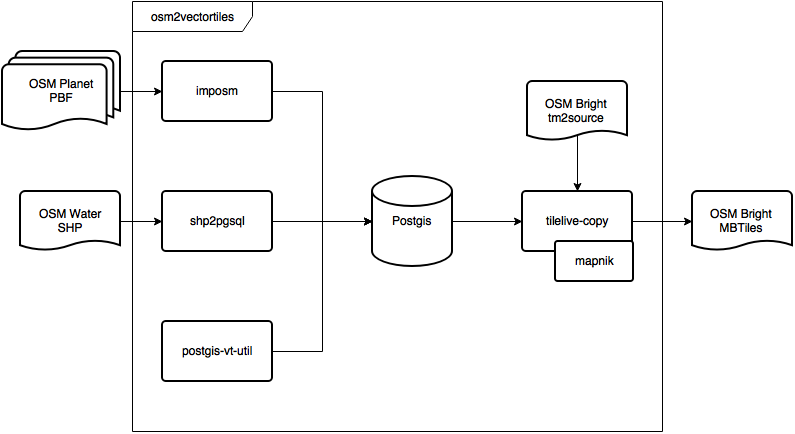
\includegraphics[width=1\textwidth]{images/osm2vectortiles.png}
  \caption{On the left side are the data sources, which get imported into a Postgis database. The import tools (imposm, shp2pgsql) map the data to a database table.
The data source (OSM bright tm2source in figure) defines different feature sets(landuse, water, roads etc.) together with a sql query.
Tilelive-copy takes the data source as input, executes the different sql queries and deliveres the queried OSM data to the mapnik rendering engine. Mapnik takes the OSM data and outputs vector tiles.
  }
\end{figure}

\section{Tile Server}

\paragraph{Visual Style} What is a visual style

\subsection{Raster Tile Server}

The raster tile server makes it possible to view the vector tiles. The output of the vector tile rendering process is just the raw vector data. To view the vector tiles we need a visual style, which defines how the defined feature sets in the data source should look like. The visual style defines for example that the feature set landuse should have a green color or that water should be blue. In the figure below we can see on the left side our vector tiles (mbtiles) and the visual style (TM2 Style). Tessera takes these two items and delivers them to mapnik which generates raster tiles. Tessera automatically starts a webserver and serves the generated raster tiles.

\begin{figure}[h]

  \centering
  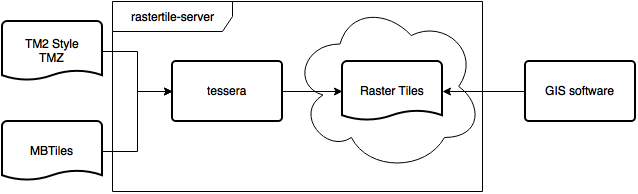
\includegraphics[width=1\textwidth]{images/rastertiles-server.png}
  \caption{Flow diagram of import and export process.}
\end{figure}

\subsection{Vector Tile Server}




\newpage